\documentclass[border=4pt,12pt]{standalone}
% House style for redrawn exam diagrams (diagram-v4: 0.4pt lines, filled -latex arrows, fine dashes; stipple and hatching drawn as real dots/lines (no PDF/SVG patterns, so they render in every browser and at any scale); transparent background). Every figure \input's this.
\usepackage{amsmath,amssymb}
\usepackage{txfonts}
\usepackage{pdfrender,xcolor}
% \halo{text}: label on shading. The shading stops just around each letter's outline (a thin knock-out that follows the
% glyphs, like the papers' typesetting), never a box. Owner: "I don't want a box around the text".
\newcommand{\halo}[1]{\leavevmode\rlap{\pdfrender{TextRenderingMode=2,LineWidth=2.2pt,LineJoinStyle=1,StrokeColor=white,FillColor=white}#1}#1}
\usepackage{tikz,pgfplots}
\pgfplotsset{compat=1.18}
\usetikzlibrary{arrows.meta,calc,angles,quotes,patterns,patterns.meta,intersections,positioning,decorations.markings,shapes.geometric}
% Stipple and hatching are drawn as actual dots / lines clipped to the region (path picture), NOT as pattern fills:
% SVG <pattern> fills vanish or blur when browsers scale the image, so the owner could not see the shading.
% Each dot is a 0.72pt square (keeps SVGs small; reads as a dot at print size). Dots sit on one global staggered grid, so neighbouring regions line up.
\makeatletter
\newdimen\ex@x \newdimen\ex@y \newdimen\ex@xa \newdimen\ex@ya \newdimen\ex@xb \newdimen\ex@yb \newcount\ex@row
\def\exam@stipplecolor{black!75}\def\exam@dotr{0.42pt}\def\exam@dotgap{2.5}
\def\ex@rowdots{\ifdim\ex@x<\ex@xb \pgfpathrectangle{\pgfqpoint{\dimexpr\ex@x-0.36pt\relax}{\dimexpr\ex@y-0.36pt\relax}}{\pgfqpoint{0.72pt}{0.72pt}}\advance\ex@x by \exam@dotgap pt\relax\expandafter\ex@rowdots\fi}
\def\exam@stipple{%
  \pgftransformreset% dots are sized in real points even inside scaled pictures
  \pgfpointanchor{path picture bounding box}{south west}\ex@xa=\pgf@x \ex@ya=\pgf@y
  \pgfpointanchor{path picture bounding box}{north east}\ex@xb=\pgf@x \ex@yb=\pgf@y
  \pgfsetfillcolor{\exam@stipplecolor}\pgfmathsetmacro\ex@h{\exam@dotgap/2}%
  \pgfmathtruncatemacro\ex@r{floor(\ex@ya/\ex@h)-1}\ex@row=\ex@r\relax
  \ex@y=\ex@r\dimexpr\ex@h pt\relax
  \loop\ifdim\ex@y<\ex@yb
    \pgfmathtruncatemacro\ex@c{floor(\ex@xa/\exam@dotgap)-1}\ex@x=\ex@c\dimexpr\exam@dotgap pt\relax
    \ifodd\ex@row \advance\ex@x by \ex@h pt\fi
    \ex@rowdots
    \advance\ex@y by \ex@h pt \advance\ex@row by 1
    \ifnum\numexpr\ex@row-(\ex@row/4)*4\relax=0 \pgfusepath{fill}\fi% flush every 4 rows: bounded TeX memory, few clip copies in the SVG
  \repeat\pgfusepath{fill}}
\newdimen\ex@d
\def\exam@hatch#1{% #1 = 1 for /, -1 for \ ; lines 45 degrees, 3pt apart
  \pgftransformreset
  \pgfpointanchor{path picture bounding box}{south west}\ex@xa=\pgf@x \ex@ya=\pgf@y
  \pgfpointanchor{path picture bounding box}{north east}\ex@xb=\pgf@x \ex@yb=\pgf@y
  \ex@d=\dimexpr\ex@yb-\ex@ya\relax \ex@x=\dimexpr\ex@xa-\ex@d\relax
  \loop\ifdim\ex@x<\ex@xb
    \ifnum#1>0 \pgfpathmoveto{\pgfqpoint{\ex@x}{\ex@ya}}\pgfpathlineto{\pgfqpoint{\dimexpr\ex@x+\ex@d\relax}{\ex@yb}}%
    \else \pgfpathmoveto{\pgfqpoint{\ex@x}{\ex@yb}}\pgfpathlineto{\pgfqpoint{\dimexpr\ex@x+\ex@d\relax}{\ex@ya}}\fi
    \advance\ex@x by 4.24pt
  \repeat
  \pgfsetlinewidth{0.4pt}\pgfsetstrokecolor{black}\pgfusepath{stroke}}
\def\examstipple{\exam@stipple}\def\examhatch{\exam@hatch}\def\examsetstipplecolor#1{\def\exam@stipplecolor{#1}}\def\examsetdotgap#1{\def\exam@dotgap{#1}}
\makeatother
% (legacy pattern kept for old files)
% staggered stipple like the NESA papers' dotted shading
\pgfdeclarepatternformonly{exam stipple}{\pgfpointorigin}{\pgfqpoint{2.2pt}{2.2pt}}{\pgfqpoint{2.2pt}{2.2pt}}{%
  \pgfpathcircle{\pgfqpoint{0.55pt}{0.55pt}}{0.42pt}\pgfpathcircle{\pgfqpoint{1.65pt}{1.65pt}}{0.42pt}\pgfusepath{fill}}
\tikzset{
  every picture/.style={line width=0.6pt, >={Latex[length=2mm,width=1.3mm]}},
  curve/.style={line width=0.6pt},
  open arrow/.style={-{Latex[length=2mm,width=1.3mm]}},  % owner: filled -latex heads everywhere, no open chevrons
  aux/.style={dash pattern=on 2pt off 1.5pt, line width=0.6pt},
  shade/.code={\def\exA{#1}\def\exB{none}\ifx\exA\exB\else\pgfkeysalso{fill=black!18}\fi},
  shade/.default=on,
  shade dots/.style={fill=none, path picture={\examstipple}},
  stipple color/.code={\examsetstipplecolor{#1}},
  stipple gap/.code={\examsetdotgap{#1}},
  shade dense dots/.style={fill=none, stipple gap=1.6, path picture={\examstipple}},
  shade hatch/.style={fill=none, path picture={\examhatch{1}}},
  shade hatch reverse/.style={fill=none, path picture={\examhatch{-1}}},
  shade solid/.style={fill=black},
  pt/.style={circle, fill, inner sep=1.1pt},
  open pt/.style={circle, draw, fill=white, inner sep=1.1pt},
}
\pgfplotsset{
  exam axes/.style={axis lines=middle, axis line style={->}, xlabel={$x$}, ylabel={$y$},
    xlabel style={anchor=west}, ylabel style={anchor=south}, tick label style={font=\small},
    every axis plot/.append style={line width=0.6pt, black}, samples=200, clip=false,
    enlargelimits=false, axis on top},
}

\begin{document}
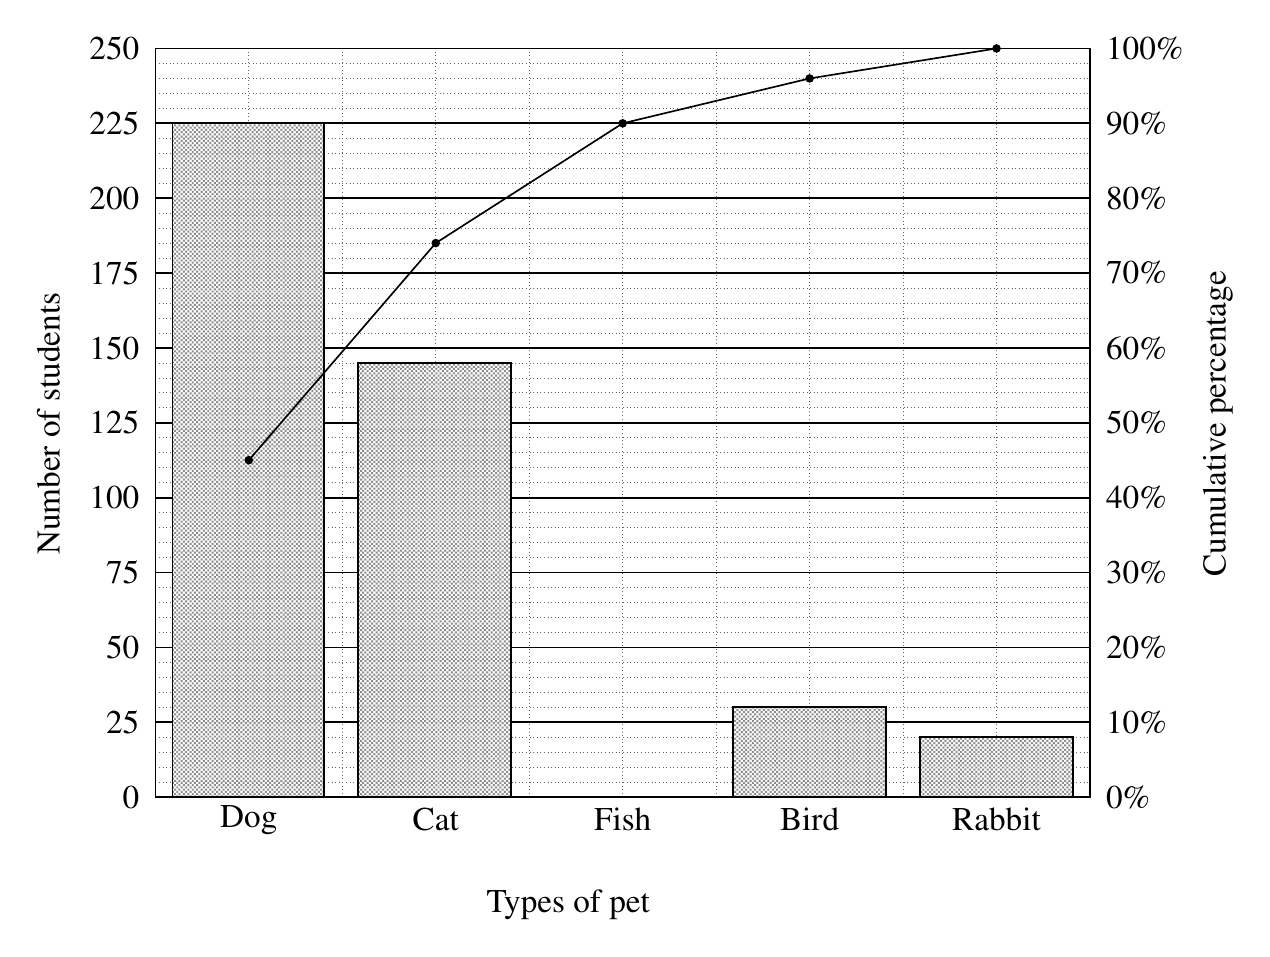
\begin{tikzpicture}[x=0.0127cm,y=-0.0127cm]
  % Pareto chart: Dog 225, Cat 145, Fish (removed; 80), Bird 30, Rabbit 20; total 500; cumulative 45,74,90,96,100%
  \draw[densely dotted,line width=0.3pt,black!60] (142,765.5) -- (1077,765.5) (142,750.5) -- (1077,750.5) (142,735.6) -- (1077,735.6) (142,720.6) -- (1077,720.6) (142,690.6) -- (1077,690.6) (142,675.6) -- (1077,675.6) (142,660.7) -- (1077,660.7) (142,645.7) -- (1077,645.7) (142,615.7) -- (1077,615.7) (142,600.7) -- (1077,600.7) (142,585.8) -- (1077,585.8) (142,570.8) -- (1077,570.8) (142,540.8) -- (1077,540.8) (142,525.8) -- (1077,525.8) (142,510.9) -- (1077,510.9) (142,495.9) -- (1077,495.9) (142,465.9) -- (1077,465.9) (142,450.9) -- (1077,450.9) (142,436.0) -- (1077,436.0) (142,421.0) -- (1077,421.0) (142,391.0) -- (1077,391.0) (142,376.0) -- (1077,376.0) (142,361.1) -- (1077,361.1) (142,346.1) -- (1077,346.1) (142,316.1) -- (1077,316.1) (142,301.1) -- (1077,301.1) (142,286.2) -- (1077,286.2) (142,271.2) -- (1077,271.2) (142,241.2) -- (1077,241.2) (142,226.2) -- (1077,226.2) (142,211.3) -- (1077,211.3) (142,196.3) -- (1077,196.3) (142,166.3) -- (1077,166.3) (142,151.3) -- (1077,151.3) (142,136.4) -- (1077,136.4) (142,121.4) -- (1077,121.4) (142,91.4) -- (1077,91.4) (142,76.4) -- (1077,76.4) (142,61.5) -- (1077,61.5) (142,46.5) -- (1077,46.5);
  \draw[densely dotted,line width=0.3pt,black!60] (235.5,780.5) -- (235.5,31.5) (329.0,780.5) -- (329.0,31.5) (422.5,780.5) -- (422.5,31.5) (516.0,780.5) -- (516.0,31.5) (609.5,780.5) -- (609.5,31.5) (703.0,780.5) -- (703.0,31.5) (796.5,780.5) -- (796.5,31.5) (890.0,780.5) -- (890.0,31.5) (983.5,780.5) -- (983.5,31.5);
  \draw (142,705.6) -- (1077,705.6) (142,630.7) -- (1077,630.7) (142,555.8) -- (1077,555.8) (142,480.9) -- (1077,480.9) (142,406.0) -- (1077,406.0) (142,331.1) -- (1077,331.1) (142,256.2) -- (1077,256.2) (142,181.3) -- (1077,181.3) (142,106.4) -- (1077,106.4);
  \fill[white] (159,780.5) rectangle (311,106.4);
  \path[shade dense dots,stipple color=black!45] (159,780.5) rectangle (311,106.4);
  \draw (159,780.5) rectangle (311,106.4);
  \fill[white] (345,780.5) rectangle (498,346.1);
  \path[shade dense dots,stipple color=black!45] (345,780.5) rectangle (498,346.1);
  \draw (345,780.5) rectangle (498,346.1);
  \fill[white] (720,780.5) rectangle (873,690.6);
  \path[shade dense dots,stipple color=black!45] (720,780.5) rectangle (873,690.6);
  \draw (720,780.5) rectangle (873,690.6);
  \fill[white] (907,780.5) rectangle (1060,720.6);
  \path[shade dense dots,stipple color=black!45] (907,780.5) rectangle (1060,720.6);
  \draw (907,780.5) rectangle (1060,720.6);
  \draw (142,31.5) rectangle (1077,780.5);
  \draw (235.5,443.4) -- (422.5,226.2) -- (609.5,106.4) -- (796.5,61.5) -- (983.5,31.5);
  \node[pt] at (235.5,443.4) {};
  \node[pt] at (422.5,226.2) {};
  \node[pt] at (609.5,106.4) {};
  \node[pt] at (796.5,61.5) {};
  \node[pt] at (983.5,31.5) {};
  \node[left,font=\large] at (136,780.5) {$0$};
  \node[left,font=\large] at (136,705.6) {$25$};
  \node[left,font=\large] at (136,630.7) {$50$};
  \node[left,font=\large] at (136,555.8) {$75$};
  \node[left,font=\large] at (136,480.9) {$100$};
  \node[left,font=\large] at (136,406.0) {$125$};
  \node[left,font=\large] at (136,331.1) {$150$};
  \node[left,font=\large] at (136,256.2) {$175$};
  \node[left,font=\large] at (136,181.3) {$200$};
  \node[left,font=\large] at (136,106.4) {$225$};
  \node[left,font=\large] at (136,31.5) {$250$};
  \node[right,font=\large] at (1083,780.5) {$0\%$};
  \node[right,font=\large] at (1083,705.6) {$10\%$};
  \node[right,font=\large] at (1083,630.7) {$20\%$};
  \node[right,font=\large] at (1083,555.8) {$30\%$};
  \node[right,font=\large] at (1083,480.9) {$40\%$};
  \node[right,font=\large] at (1083,406.0) {$50\%$};
  \node[right,font=\large] at (1083,331.1) {$60\%$};
  \node[right,font=\large] at (1083,256.2) {$70\%$};
  \node[right,font=\large] at (1083,181.3) {$80\%$};
  \node[right,font=\large] at (1083,106.4) {$90\%$};
  \node[right,font=\large] at (1083,31.5) {$100\%$};
  \node[font=\large] at (235.5,803) {Dog};
  \node[font=\large] at (422.5,803) {Cat};
  \node[font=\large] at (609.5,803) {Fish};
  \node[font=\large] at (796.5,803) {Bird};
  \node[font=\large] at (983.5,803) {Rabbit};
  \node[font=\large,rotate=90] at (35,407) {Number of students};
  \node[font=\large,rotate=90] at (1205,407) {Cumulative percentage};
  \node[font=\large] at (555,888) {Types of pet};
\end{tikzpicture}
\end{document}
